%\wgnote{Move the followings to appendix}
%\appendix
% \chapter{Appendix}
\begin{figure*}[]
  \centering
\begin{subfigure}{0.25\textwidth}
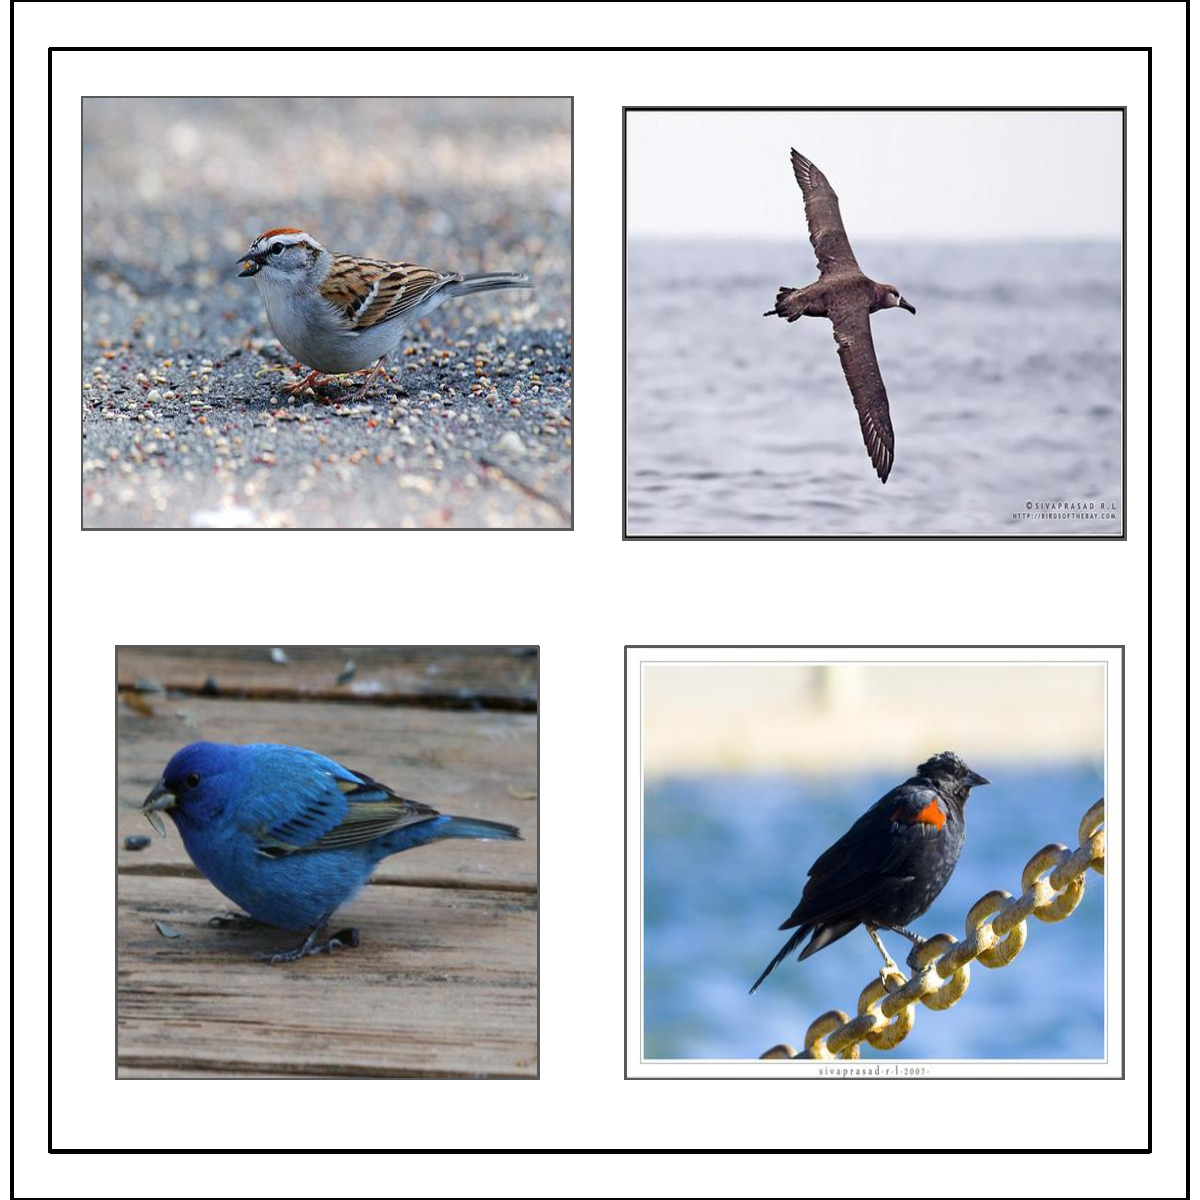
\includegraphics[width=\textwidth]{figures/Figure_3A.pdf}
  \subcaption{CUB dataset.}
\end{subfigure}
\hspace{0.04\textwidth}
% <— this is important. There should be no empty line here. 
\begin{subfigure}{0.25\textwidth}
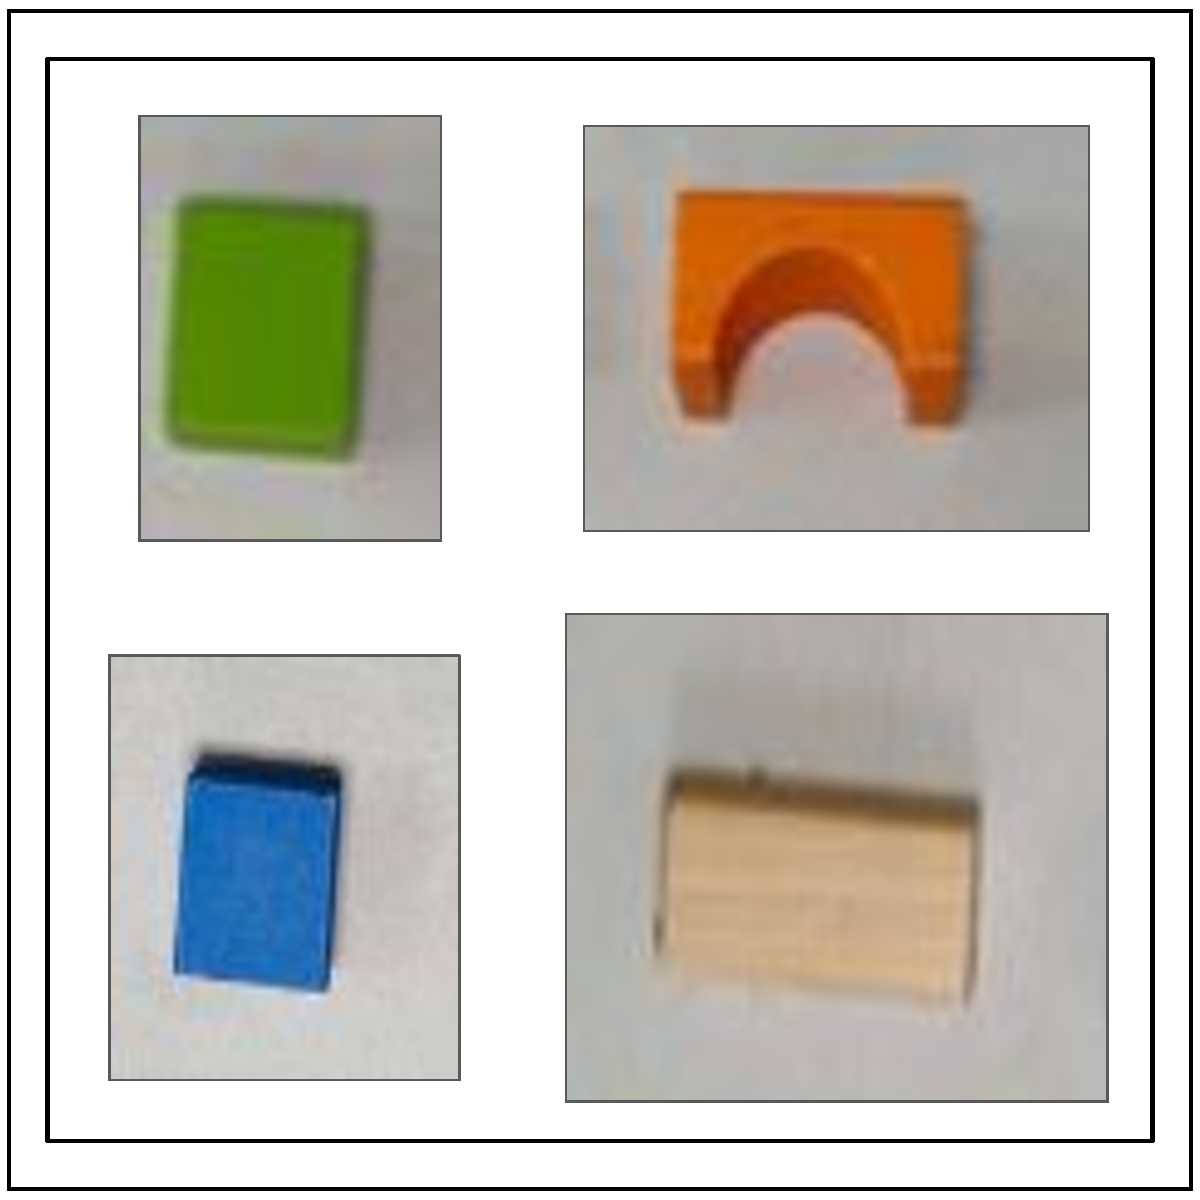
\includegraphics[width=\textwidth]{figures/Figure_3B.pdf}
  \subcaption{House construction domain}
\end{subfigure}
\hspace{0.04\textwidth}
%
\begin{subfigure}{0.25\textwidth}
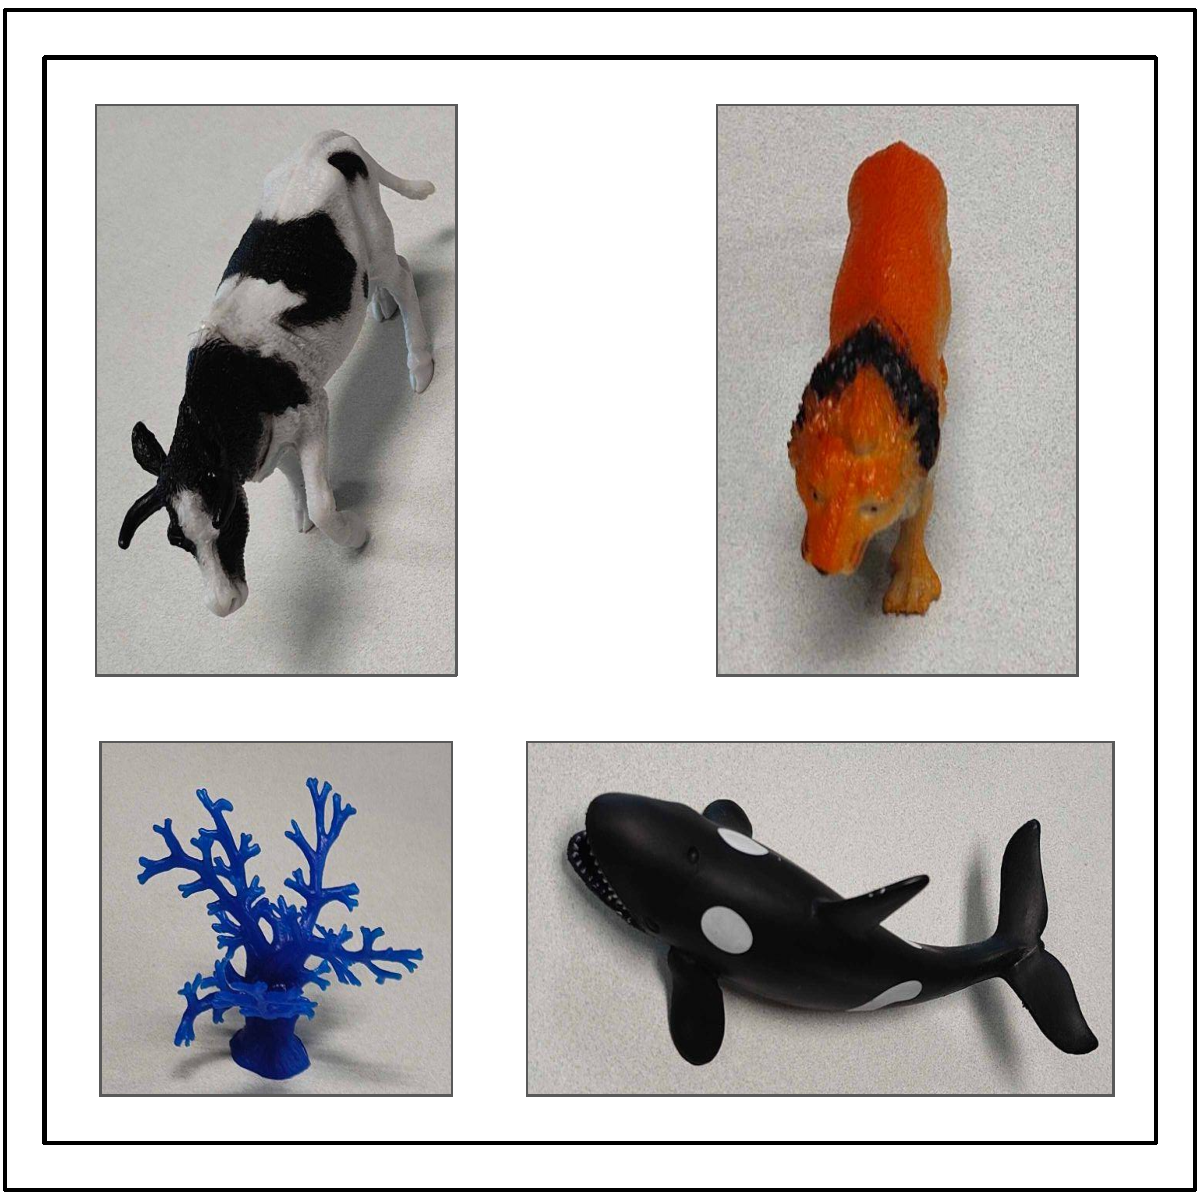
\includegraphics[width=\textwidth]{figures/Figure_3C.pdf}
  \subcaption{Zoo domain}
\end{subfigure}
\caption{Sample images from the three domains in this work.}
\label{fig:sampled_figures}
\end{figure*}


% \subsection{Node Classifier}
% Figure~\ref{fig:node_classifier} describes the process of how our pipeline choose an object to pick. 
% The inference is a two-step process, both using a BERT\textsubscript{base} model and a MLP layer, and taking the node context $t_i$ and he linguistic request $q$ as inputs.
% In the first step we use the BERT\textsubscript{base} model and a MLP layer to decide whether the node in the goal graph is different from the corresponding node in the demonstration. 
% Then we use another BERT\textsubscript{base} model and MLP layer to extract the object from $t_i$ and $q$ for this node location.

% In the example of Figure~\ref{fig:node_classifier}, we are trying to decide the object that should be placed in position $5$.
% Based on the node context $t_5$ and the request $q$, the node classifier decides that node $5$ in the goal graph should remain the same as the demonstration. 
% Then, we use the concept extractor to extract the object from $t_5$, and we found that the object that should be placed at node $5$ is ''blue rectangular tile''.

\subsection{Training Pipeline}
 We explain our training pipeline in this section. 
 The concepts from the dataset is divided into three groups: $C_{pretrain}, C_{train}$ and $C_{test}$, where the pre-train concepts $C_{pretrain}$ represent the pre-existing nodes in the knowledge graph. The training of the concept net model consists of three stages, the pre-training for the visual feature extractor, the pre-training for the embedding of pre-train concepts $C_{pretrain}$, and the training to update the knowledge graph with train concepts $C_{train}$. 
 \paragraph{Pre-training the Visual Feature Extractor.}
 In the first pre-training stage, we generate a VQA dataset on both the pre-train concepts $C_{pretrain}$ and the train concepts $C_{train}$. The purpose of this stage is to expose the visual feature extractor with a larger variation of visual features. 
 We jointly pre-train the visual feature extractor and the embedding for the pre-train concepts $C_{pretrain}$ and the train concepts $C_{train}$ with the visual question-answering task in this stage.
 After this pre-training stage, the embeddings of all pre-train concepts and train concepts will be discarded.
 \paragraph{Pre-training Pre-train Concepts.}
 The embedding of pre-train concepts $C_{pretrain}$ is obtained through gradient descent in this pre-train phase.
 For this phase, we generate a VQA dataset on the pre-train concepts $C_{pretrain}$ only.
 After we warmup the visual feature extractor in the first pre-training phase, we jointly train the visual feature extractor and the embedding for the pre-train concepts in this phase using the same VQA task.
 This pre-training step is skipped under the setting where the concept net has zero prior knowledge of the concepts, which is the setting of all of our experiments.
 \paragraph{Training.} 
 After we have pre-trained the visual feature extractor and the embedding for the pre-train concepts,  we train the concept learner module during the training stage.  We freeze the weights of the visual feature extractor at this stage because otherwise the embeddings for the pre-train concept will not be usable.  Because we hope to train ARGNN to update the embedding for known concepts with information from unseen instances, we have to reset the embedding for all the pre-train concepts and train concepts,$C_{pretrain}$ and $C_{train}$, after all the train concepts are inserted to the network.  After inserting all the concepts within the train set in the final round, we do not reset the embedding for the train concepts and insert the concepts in the test set $C_{test}$. 

\subsection{Training Configurations}
In this section we describe the training configuration of the experiments for all the three domains. 
During the training phase, the model completes one round of training if it finishes to insert all the concepts in the training set once. For simplicity, we unify the steps of training with rounds of insertion.
For all the experiment results we report in this work, we adopted the configuration where there is no pre-train concepts.
As a results, the second phase of pre-training is skipped for all the three datasets.
For all the three domains, we train our model for completing the concept graphs 100 rounds, and the number of concept insertions varies depending on the split of the concepts. We start the training with a learning rate of 0.001 and decrease the learning rate by a factor of 0.1 in every 25 rounds of completing the knowledge graph in the training stage.
For CUB-200-2011 dataset, we train our model for 50000 iterations with a batch size of 10. We use an Adam optimizer with learning rate of 0.0001 in the pre-training phase of the visual feature extractor.
For the house construction domain and the zoo domain, we train our model for 5000 iterations with a batch size of 10. We use an Adam optimizer with learning rate of 0.0001 in the pre-training stage of the visual feature extractor.

\subsection{Robot Setup}
We describe the details for camera calibration.
We need to calibrate cameras with respect to the FR3 base frame. 
We take multiple pictures in different configurations of the FR3 end-effector to which an acuro market is attached. This allows us to find a transformation matrix which converts the coordinates from the  camera frame to the robot base frame. The place scene camera is used to find the length of the object occupying the current node of the scene graph. 

We describe how we compute the placement location for each object in detailed.
SAM is used to segment the objects placed in the place scene and find the bounding boxes of each placed object which are also the nodes of our scene graph.
This allows us to calculate the position of the next object by finding the relative position of the next node with respect to the current object being placed.
, referencing the position of the node of the scene, and calculating the length of the bounding box of the referenced node. 
we use a formula of shift = 1/2*max(bounding box of the referenced node length)+50 pixel space \textbf{Next node position}= Relation to the reference node(Reference node position,shift). The function relation to the reference node adds a shift to the reference node position based on its relation to the next node. For example, it adds the shift only to the x coordinate if there is "to the top of" relation, or in the case of "to the right of" relation, it adds only the y coordinate of the current position. In our scene graph, we are able to identify "to the top of ", "to the bottom of"," to the right of"," to the left of", "to the top right of"," to the top left of"," to the bottom right of", and "to the bottom left of" relations.\\
The Segment Anything Model is capable of separating the foreground from the background. This allows us to find the table mask and the segment of each object placed in the camera frame on the table. \\
The flow of our pipeline requires us to first demonstrate the visual scene with all the objects placed in the Task scene to make a structure with linguistic inputs. 
We have to make sure that the objects are placed at a distance that allows SAM to create separate segment boxes for the objects. Then we pass each segmented object to either FALCON or Hi-Viscont classifiers to classify conditioned on the given language query. The robot then picks the object with simple visuo-motor servoing. 
by the node information of the scene graph. 
Once we find the object to be picked we then calculate the center of the bounding box of that object and convert it to the Robot frame with the help of the transformation matrix. 
If in the process there is an incomplete or erroneous grasp, we reattempt the whole classification again autonomously. Once the object is grasped we then place the object into the Task scene, with the position calculated relatively 
with respect to the previously placed object nodes or the ground. This process is iteratively done until we have completed the whole scene graph.
%\asnote{nodes in place of node or the ground} or \ngnote{the ground object}. 

